% !TeX root = Report.tex

\section{Predicates}

When considering how to evaluate predicates there are many points that need to be considered. Depending on what the intention is certain implementations of predicate evaluation are going to be better than other implementations. Also, when developing with considerations of the predicate evaluation such as accuracy, the considerations of sensor networks will need to be taken into account (such as the minimisation of energy usage). This section will first detail the types of predicates that we identify that we wish to be able to detect, then it will cover how we can evaluate such predicates and finally will discuss several implementations of transmitting the information to the required part of the network.

\subsection{Types of Predicates}

In the introduction several different classes of predicates were discussed, of which the most important one to us is the locality of the predicate. A majority of the work focuses on global predicates \cite{277788,345831,553309} which while useful in general for distributed systems is perhaps not as helpful for wireless sensor networks. To begin with many of the problems that a sensor network may encounter are local problems. By local we mean that a node in the network only has access to a specific subset of the networks information, in our case we focus on the surrounding neighbours of the node evaluating the predicate. When forcing a local problem to be evaluated globally it means that investigating evaluating that predicate locally is eliminated. This is problematic as there may be energy savings when evaluating a predicate locally. So the first major decision is that instead of focusing on global predicates, local predicates are instead the focus - in order to investigate any potential energy savings.

\begin{mydef}
\emph{Global Predicate}: A predicate $P$ that operates on some global state $S$ where $S$ is a mapping from a node id to some data on that node.
\end{mydef}

\begin{mydef}
\emph{Local Predicate}: A predicate $P$ evaluated on the node $j$, where the state $N(j, n) \subseteq S$ available contains information on some $n$-hop neighbourhood of $j$. Where $N(j, n)$ is a function that returns the state of all nodes within $n$ hops of $j$.
\end{mydef}

The second decision is to decide on is the stability of the predicate being detected. As discussed in the introduction there is a choice between stable predicates that remain true and unstable predicates whose truth value can alternate. This decision is important because it will affect the algorithm structure, an example of this is that taking snapshots of global state and checking the predicate against that works for checking stable predicates. However, for unstable predicates detailed recording of the traces of the system is required \cite{bansod2004distributed}. Due to the limited resources of sensor nodes we focus on the simpler problem of stable predicates. This is mainly because complex programs tend to require a greater number of instructions to do more things and the size of the firmware on the motes is limited \cite{CM5000}.


\begin{mydef}
\emph{Application Predicate}: A predicate that is evaluated over the state an application is in. This can involve extracting and examining sensor data or program variables.
\end{mydef}

\begin{mydef}
\emph{Network Predicate}: A predicate that is evaluated over the network interactions. Examples include detecting collisions where there should have been none, or checking that there are no loops in multi-hop communications.
\end{mydef}

So far traditional predicate properties have been focused on. However, we need to introduce two new classes of predicates. In previous work the authors dealt in the abstract notion of program traces, these traces are simply events that lead to some eventual state. When developing software for sensor networks we feared that (i) the hooks to detect the traces and (ii) record them would be too demanding on the limited resources. By considering what happens in the application separately from the network the impacts may be decreased. Network predicates would involve monitoring the low level MAC layer for network events and also including extra data to packets sent from the node. Application predicates could imply be evaluated instantaneously on the data available. Due to the simplicity, but the good results that application predicates may provide we focus solely on them.

Much of the previous work exists in ideal worlds were assumptions such as ``no messages are lost'' \cite{277788} are made. Unfortunately this is not the case in the real world, while the MAC layer and the application layer can do much to mitigate packet loss \cite{Buettner:2006:XSP:1182807.1182838} without energy expensive protocols such as 802.11 which use a MAC protocol based on CSMA/CA \cite{?} it is not possible to ensure a certain level of reliability. Therefore it must be realised that every time a predicate is evaluated it will have a certain level of accuracy. This is because some data may have been lost on the way to its destination or outdated information was used. We believe the accuracy is a very important angle to predicate evaluation as an accurate predicate evaluation that is not received often will inform the systems user more than a predicate evaluation result that is received very frequently but is also very inaccurate.

In summary we focus on evaluating predicates that are stable and use local information. These predicates also deal excursively with information about the application running on the mote and not the communication it is involved with. Also there should be a focus that predicates are evaluated as accurately as possible with a minimum amount of energy. The next two sections will detail how predicates are evaluated in our implementation and then how the required information is disseminated to the correct motes.

\subsection{Predicate Evaluation}

When deciding how we would evaluate predicates once data was received there were two possible solutions that were considered. The first was to simply have the system developer hardcode the checking into the code and provide a library to handle responses, the second was to implement a virtual machine that would run a script that checks the predicate. Using hard checks written in C would have provided a more efficient way of checking the predicate and would be similar to the approach used by HSend \cite{herbert2007adaptive} which parsed the C source code and generated C code for the predicates specified in a special comment block. A downfall of hardcoding the predicate evaluation is that it could lead to a large inflation of the firmware and if the system developers wanted to change, add or remove a predicate then they would need to update the entire firmware image across the network \cite{Dunkels:2006:RDL:1182807.1182810,1437066}.

With a scripting language, instead of sending a large firmware binary across the network a small program of high level opcodes could be sent instead. The difference could be huge, for example the maximum firmware size of the CM5000 is 48KB \cite{CM5000}, and it is conceivable that a program script utilising high level instructions could instead fit into the size of a single packet (128 bytes\footnote{\url{http://contiki.sourceforge.net/docs/2.6/a00302.html}}). Therefore to aid in the flexibility of our solution we implemented a simple virtual machine and language that was executed to evaluate the predicate.


Initially we looked for an already developed scripting language that we could use on the motes. Having used high level scripting languages such as Python and Lua we first looked into using them. Unfortunately even though Lua offered an embedded alternative called eLua \cite{elua} the firmware size and the RAM usage would have been unacceptably high for the hardware at our disposal. We then started looking at a language called SCript  \cite{dunkels06lowoverhead} by  \citeauthor{dunkels06lowoverhead} who was also the author of Contiki, the wireless sensor network OS we were using. Unfortunately (in part due to the name) we were unable to find the implementation of it. Finally we looked at Antelope \cite{Tsiftes:2011:DS:2070942.2070974} which provided a way to query nodes using SQL like a database. Unfortunately we were unsure as to how much control we would have on being able to optimise energy usage via different ways of gathering data. So we concluded that we would need to create our own language, parser for it, assembler and virtual machine to execute the produced code.


The predicate evaluation language that we designed needed to be fairly simple to make it (i) easy to implement and (ii) easy to execute. To do this we set out a number of desired features and then explicitly decided on features that would not be included because of their irrelevance as can be seen in \autoref{tab:language-requirements}. The most important feature was that we wanted to be able to test a sub-predicate over a set of neighbouring node's data, this meant that we would need a way to represent a set of data and iterate over it. As the program is always intended to return a boolean result, there was no need to implement comprehensive iteration of the form \verb|for (<INIT>; <CONTINUE>; <NEXT>)| we instead could just implement forall and exists operators. To simplify further the language was designed to be functional rather than imperative as we had no need for our predicate checker to directly cause state changes in the application running directly on the hardware.

We managed to implement the majority of the features we desired, however there were some that were difficult to implement or had to be implemented differently. The first is feature 4 (set operations), which simply would have been too difficult to implement and would have greatly increased the code size. The next is feature 6 (targeting multiple nodes), this was not implemented because it would have required a variable amount of space in the message that disseminated the predicate throughout the network. There is also a simple work around, which is to create a new predicate using the same code for each of the nodes that wish to be targeted.

For some of the features we desired we ended up implementing them differently than expected. Initially we expected to allow users to define functions and structures that could be operated on (like in C). However, what we ended up with was slightly different. We ended up with a primitive called \verb|Neighbours(n)| which allowed the predicate to ask for its $n$-hop neighbourhood, we also ended up with a single structure which the user defined themselves in C and provided functions to access data in that structure. These functions are then exposed to the predicate language. Finally information on a node is only exposed to the predicate if the user provides some way to store this data in the nodes data structure and provides functions to access it. These functions and the user data structure will be explained further on.


\begin{table}[H]
\centering
\begin{tabular}{| l | l | l | l |}
\hline
\# & Feature & Desired & Implemented \\
\hline
1 & Integer ($+$ $-$ $\times$ $\div$ $=$ $\neq$ $<$ $\leq$ $>$ $\geq$ casts) & Yes & Yes \\
2 & Floating Point ($+$ $-$ $\times$ $\div$ $=$ $\neq$ $<$ $\leq$ $>$ $\geq$ casts) & Yes & Yes \\

3 & Set iteration support ($\forall$ $\exists$) & Yes & Yes \\
4 & Set operation support ($\cup$ $\cap$ $\setminus$ $\{\}$) & Yes & No \\

5 & Ability to specify predicate target(s) (Single or Every node) & Yes & Yes \\
6 & Ability to specify predicate target(s) (Multiple nodes) & Yes & No \\

7 & Ability to get the current node information ($this$) & Yes & Yes \\

8 & Limited function support (eg. $Neighbourhood(N, H)$) & Yes & Partial \\
9 & Limited structure support (eg. $N.Temperature$) & Yes & Partial \\

10 & Ability to get sensor information on a node & Yes & Partial \\
11 & Ability to get node information (Distance to Sink, \ldots) & Yes & Partial \\

12 & Strings & No & No \\
13 & IO & No & No \\

14 & Data structures (Lists, Arrays, Dictionaries, \ldots) & No & No \\
15 & Library features (Custom libraries or built-in libraries) & No & No \\
16 & Interactive mode (terminals) & No & No \\
\hline
\end{tabular}
\caption{Predicate Language Features}
\label{tab:language-requirements}
\end{table}

The major problem with developing our own language was that we needed a way to convert that into a compact form that could be easily executed by a virtual machine. As can be seen by the complexities of the GCC and LLVM/Clang projects, compilation of abstract code to optimal executable code is a difficult problem. So instead of trying to develop a highly optimising compiler, our target was to develop a compiler that produced good code that was capable of being hand optimised by developers before being deployed to the network.

To reach this goal, we followed good development principles and broke down the creation of this executable code into to separate phases: the compiler and the assembler. The compiler parsed the predicate language and compiled it down to a human readable intermediate representation (IR) that could be understood and modified by humans. The assembler then converted this into the raw bytecode that would be sent to the motes for evaluation. Having a human readable IR makes hand--optimisation very simple, and easy to support directly within the visualisation tool. This separation leads to the workflow of developing and deploying a predicate as shown in \autoref{fig:pred-workflow}.

\begin{figure}[H]
\centering
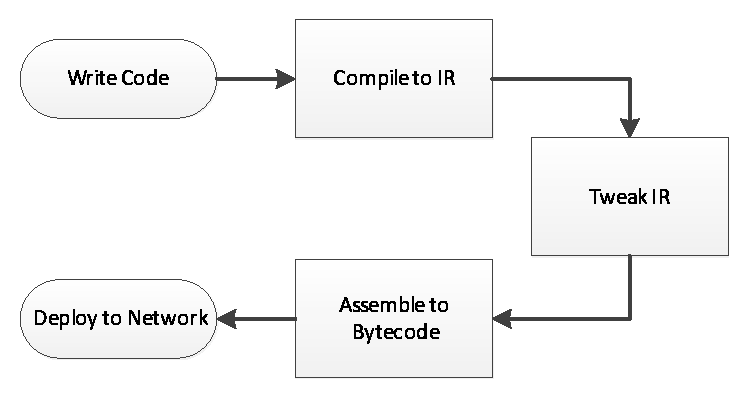
\includegraphics{Diagrams/predicate-dev-process.eps}
\caption{Workflow to create and deploy a user written predicate}
\label{fig:pred-workflow}
\end{figure}


\subsubsection{Domain Specific Language}

The following is the definition of how to parse our predicate language. We implemented it in Java using JavaCC, using several resources \footnote{JavaCC tutorial: \url{http://cs.lmu.edu/~ray/notes/javacc/}} to help in the development. In the language there are four main components. The first is the target of the predicate specified within square brackets, the target can be a node address (such as 1.0) or `all' to target all nodes in the network. The second is the function definitions. When users initialise our library on the motes, they need to provide a function that provides the current information on the node and a mapping of function ids to the functions used to access this data. The function definition statement in the predicate language allows a human understandable name to be assigned to a function id and it also tells the compiler what id function should be called and the type that that function returns. The third is the `using' statement that allows a set of neighbouring information to be assigned to a variable name. This is the only way to request node information not about the current node that is evaluating the predicate. The fourth and final part if the predicate itself, which includes expected logic operators that operate over sets, integers, floating point numbers and booleans. The logical operators that make up the predicate are described in \autoref{tab:lang-operators}.


\begin{table}[H]
\centering
\begin{tabular}{| l | l | l | l | l |}
\hline
Name & Logic & Symbol & Input Type(s) & Output Type\\
\hline

For All & $\forall$ & \sm{@} & Set of user defined data & Boolean\\
Exists & $\exists$ & \sm{\#} & Set of user defined data & Boolean\\

\hline

And & $\land$ & \sm{\&} & Booleans & Boolean\\
Or & $\lor$ & \sm{\textbar} & Booleans & Boolean\\
Xor & $\oplus$ & \sm{\textasciicircum} & Booleans & Boolean\\
Implies & $\implies$ & \sm{=\textgreater} & Booleans & Boolean\\
Equivalence & $\iff$ & \sm{\textless=\textgreater} & Booleans & Boolean\\

\hline

Not & $\lnot$ & \sm{!} & Boolean & Boolean\\

\hline

Equality & $=$ & \sm{==} & Integers or Floats & Boolean\\
Inequality & $\not=$ & \sm{!=} & Integers or Floats & Boolean\\
Less Than & $<$ & \sm{\textless} & Integers or Floats & Boolean\\
Less Than or Equal To & $\leq$ & \sm{\textless=} & Integers or Floats & Boolean\\
Greater Than & $>$ & \sm{\textgreater} & Integers or Floats & Boolean\\
Greater Than or Equal To & $\geq$ & \sm{\textgreater=} & Integers or Floats & Boolean\\

\hline

Addition & $+$ & \sm{+} & Integers or Floats & Integer or Float\\
Subtraction & $-$ & \sm{-} & Integers or Floats & Integer or Float\\
Multiplication & $\times$ & \sm{*} & Integers or Floats & Integer or Float\\
Division & $\div$ & \sm{/} & Integers or Floats & Integer or Float\\

\hline
\end{tabular}
\caption{Logical operators implemented in predicate language}
\label{tab:lang-operators}
\end{table}

\begin{figure}[H]
\begin{eqnarray*}
	\pn{eval} & \pp & [ \pn{target} ] \ww \pn{function} \\
	\pn{target} & \pp & \smlst{all} \\
	~ & \oo & \pn{number}\sm{.}\pn{number} \\
%
	\pn{function} & \pp & \smlst{function} \ww \pn{number} \ww \smlst{as} \ww \pn{string} \ww \smlst{returning} \ww \pn{type} \ww \smlst{in} \ww \pn{function} \\
	~ & \oo & \pn{using} \\
%
	\pn{using} & \pp & \smlst{using} \ww \smlst{Neighbours}\sm{(}\pn{number}\sm{)} \ww \smlst{as} \ww \pn{variable} \ww \smlst{in} \ww \pn{using} \\
	~ & \oo & \pn{predicate} \\
%
	\pn{predicate} & \pp &  \sm{(}\pn{predicate}\sm{)} \\
	~ & \oo & \pn{quantifier}\sm{(}\pn{variable} \ww \sm{:} \ww \pn{variable} \ww \sm{\mytilde} \pn{predicate} \sm{)}\\
	~ & \oo &  \pn{predicate} \ww \pn{logical-binary} \ww \pn{predicate} \\
	~ & \oo &  \pn{logical-unary} \ww \pn{predicate} \\
	~ & \oo &  \pn{var-expr} \ww \pn{math-logical-binary} \ww \pn{var-expr} \\
%
	\pn{var-expr} & \pp & \sm{(}\pn{var-expr}\sm{)} \\
	~ & \oo & \pn{number} \\
	~ & \oo & \pn{string}\sm{(}\pn{this-variable}\sm{)} \\
	~ & \oo & \pn{var-expr} \ww \pn{math-binary} \ww \pn{var-expr} \\
	~ & \oo & \smlst{abs}\sm{(}\pn{var-expr}\sm{)} \\
	~ & \oo & \pn{set-fn}\sm{(}\pn{variable}\sm{)} \\
	~ & \oo & \pn{transform-set-fn}\sm{(}\pn{transform-fn}\sm{,} \ww \pn{variable}\sm{)} \\
%
	\pn{this-variable} & \pp & \pn{variable} \oo \smlst{this} \\
	\pn{variable} & \pp & \pn{string} \\
%
	\pn{transform-fn} & \pp & \pn{string} \\
	\pn{transform-set-fn} & \pp & \smlst{sum} \oo  \smlst{mean} \oo \smlst{max} \oo \smlst{min} \\
	\pn{set-fn} & \pp & \smlst{len} \\
%
	\pn{type} & \pp & \smlst{float} \oo \smlst{int} \\
%
	\pn{logical-binary} & \pp & \sm{\&}  \oo \sm{\textbar} \oo \sm{\textasciicircum} \oo \sm{=\textgreater} \oo \sm{\textless=\textgreater} \\
	\pn{logical-unary} & \pp & \sm{!} \\
	\pn{math-logical-binary} & \pp & \sm{==} \oo \sm{!=} \oo \sm{\textless} \oo \sm{\textless=} \oo \sm{\textgreater} \oo \sm{\textgreater=} \\
	\pn{math-binary} & \pp & \sm{+} \oo \sm{-} \oo \sm{*} \oo \sm{/} \\
%
%	\pn{string} & \pp & \pn{alpha}\pn{string-rest} \\
%	\pn{string-rest} & \pp & \nn \oo \pn{alpha}\pn{string-rest} \oo \pn{digit}\pn{string-rest} \\
%
%	\pn{alpha} & \pp & \sm{A}\dots\sm{Z} \oo \sm{a}\dots\sm{z} \\
%	\pn{number} & \pp & \pn{sign} \pn{number-first} \oo \pn{number-first} \\
%	\pn{number-first} & \pp & \pn{digit} \oo \sm{1}\dots\sm{9}\pn{number-rest} \\
%	\pn{number-rest} & \pp & \pn{digit} \oo \pn{digit}\pn{number-rest} \\
%	\pn{digit} & \pp & \sm{0}\dots\sm{9} \\
%	\pn{sign} & \pp & \sm{+} \oo \sm{-} \oo \nn \\
	\pn{quantifier} & \pp & \sm{@} \oo \sm{\#} \\
\end{eqnarray*}
\caption{Language definition}
\end{figure}

When we were implementing the parsing for the predicate language one of the major issues encountered was that parsing infix operators (that is the operator is between two operands) was much harder to accomplish than prefix or postfix operators, \cite{ParsingRecursiveDescent} was used as a guide to implement infix parsing.

Another important issue to mention is the distinction between syntax and semantics. The language definition specifies the syntax, but it fails to capture some of the semantic subtleties of valid programs. One example is that even if a variable name or a function name are syntactically valid strings, compilation should fail if they have not been defined by a statement prior to their usage. However, JavaCC provides a very capable framework for validating semantics during construction of the program's IR.

\subsubsection{Example Predicates}
\label{sec:example-predicates}

\begin{figure}[H]
\begin{minipage}{.5\linewidth}
\begin{lstlisting}[language=Hoppy]
[all]
function 1 as slot returning int in
    using Neighbours(2) as twohopn in
        @(x : twohopn ~
            slot(x) != slot(this)
        )
\end{lstlisting}
\end{minipage}%
\begin{minipage}{.5\linewidth}
\begin{align*}
&				\forall n \in \text{Nodes} \cdot \\
& \hspace{2em}		\forall n' \in \text{Neighbours}(n, 2) \cdot \\
& \hspace{4em}				\text{slot}(n) \neq \text{slot}(n')
\end{align*}
\end{minipage}

\caption{Check that no two neighbours have the same slot (2-hop information)}
\label{fig:two-hop-slot-pred-lang}
\end{figure}

\begin{figure}[H]
\begin{minipage}{.5\linewidth}
\begin{lstlisting}[language=Hoppy]
[all]
function 0 as addr returning int in
function 1 as slot returning int in
    using Neighbours(1) as onehopn in
        @(a : onehopn ~
            @(b : onehopn ~ addr(a) != addr(b)
                => slot(a) != slot(b))
            & slot(a) != slot(this)
        )
\end{lstlisting}
\end{minipage}%
\begin{minipage}{.5\linewidth}
\begin{align*}
&				\forall n \in \text{Nodes} \cdot \\
& \hspace{2em}		\forall n' \in \text{Neighbours}(n, 1) \cup \{n\} \cdot \\
& \hspace{4em}			\forall n'' \in \text{Neighbours}(n, 1) \cup \{n\} \cdot \\
& \hspace{6em}				\text{addr}(n') \not= \text{addr}(n'') \\
& \hspace{8em}					\implies \text{slot}(n') \neq \text{slot}(n'')
\end{align*}
\end{minipage}
\caption{Check that no two neighbours have the same slot (1-hop information)}
\label{fig:one-hop-slot-pred-lang}
\end{figure}


The predicates specified in \autoref{fig:two-hop-slot-pred-lang} and \autoref{fig:one-hop-slot-pred-lang} aim to check that slot allocation is correct and will not lead to collisions. As these are applications predicates they check that there are no clashes with the slots assigned. If we were also checking network related state, these predicates would also need to be monitoring the MAC layer to make sure that no collisions did in fact occur. Predicates similar to these appear in the problem statement of \cite{DBLP:journals/corr/abs-0808-0920}, which leads us to believe that an implementation of a TDMA algorithm may desire some checking of these predicates to test correctness of such an algorithm.

\begin{figure}[H]
\begin{minipage}{.5\linewidth}
\begin{lstlisting}[language=Hoppy]
[1.0]
function 3 as humidity returning float in
    humidity(this) <= 40.0
\end{lstlisting}
\end{minipage}%
\begin{minipage}{.5\linewidth}
\begin{align*}
&				\forall n \in Nodes \cdot \\
& \hspace{2em}		\text{addr}(n) = 1.0 \implies \\
& \hspace{4em}			\text{humidity}(n) \leq 40
\end{align*}
\end{minipage}
\caption{Check that the relative humidity of node 1.0 is less than or equal to 40\%}
\label{fig:app1-pred-lang}
\end{figure}

\begin{figure}[H]
\begin{minipage}{.5\linewidth}
\begin{lstlisting}[language=Hoppy]
[all]
function 2 as temperature returning float in
    using Neighbours(2) as twohopn in
        abs(temperature(this) - mean(temperature, twohopn)) <= 10
\end{lstlisting}
\end{minipage}

\begin{minipage}{.5\linewidth}
\begin{align*}
&				\forall n \in \text{Nodes} \cdot \\
& \hspace{2em}		\left|\text{temperature}(n) - \frac{\sum\limits_{n' \in \text{Neighbours}(n, 2)} \text{temperature}(n')}{|\text{Neighbours}(n, 2)|} \right| \leq 10
\end{align*}
\end{minipage}
\caption{Check that the average neighbour temperature is with 10 degrees of ours}
\label{fig:app2-pred-lang}
\end{figure}

The two predicates in \autoref{fig:app1-pred-lang} and \autoref{fig:app2-pred-lang} capture what system users may be trying to detect. \autoref{fig:app1-pred-lang} shows a predicate that fails when the humidity sensed by a predicate falls low and \autoref{fig:app2-pred-lang} detects when there is a large different in the temperature of one node and the average of its neighbours. Both of these predicates could be used when monitoring the environment in a forest to see how likely and where forest fires may be starting. 


\begin{figure}[H]
\begin{minipage}{.5\linewidth}
\begin{lstlisting}[language=Hoppy]
[all]
function 0 as addr returning int in
    using Neighbours(1) as onehopn in
    using Neighbours(2) as twohopn in
        @(a : onehopn ~
            #(b : twohopn ~ addr(a) == addr(b))
        )
\end{lstlisting}
\end{minipage}%
\begin{minipage}{.5\linewidth}
\begin{align*}
&				\forall n \in \text{Nodes} \cdot \\
& \hspace{2em}		\{\text{addr}(n') | n' \in \text{Neighbours}(n, 1)\} \subseteq \\
& \hspace{4em}			\{\text{addr}(n') | n' \in \text{Neighbours}(n, 2)\}
\end{align*}
\end{minipage}
\caption{Check 1-hop neighbourhood is in 2-hop neighbourhood}
\end{figure}

This predicate is perhaps not as interesting as other predicates but it has a valid use in testing certain aspects of the information dissemination aspect of our predicate checking algorithm. It is important that we can test our mechanisms to evaluate predicates, because if we cannot rely on the correct evaluation of predicates, then we cannot rely on the results. Predicates like checking the 1-hop neighbourhood is in the 2-hop neighbourhood allows us to check that we are gathering data in the right way.


\begin{figure}[H]
\begin{lstlisting}[language=Hoppy]
[all]
function 5 as sink-distance returning int in
    using Neighbours(1) as onehopn in
        sink-distance(this) == min(sink-distance, onehopn) + 1
\end{lstlisting}
\caption{We are one hop further from the base station than the closest of our neighbours. May be used to check parent in aggregation tree is actually closer to the sink.}
\label{fig:tree-agg-parent-hops-pred-lang}
\end{figure}

\begin{figure}[H]
\begin{minipage}{.5\linewidth}
\begin{lstlisting}[language=Hoppy]
[all]
function 0 as addr returning int in
function 4 as ch returning int in
function 6 as H returning int in
    using Neighbours(H(this)) as neighbours in
        #(node : neighbours ~
            ch(this) == addr(node)
        )
\end{lstlisting}
\end{minipage}%
\begin{minipage}{.5\linewidth}
\begin{align*}
&				\forall n \in \text{Nodes} \cdot \\
& \hspace{2em}		\exists n' \in \text{Neighbours}(n, \text{H}(n)) \cdot \\
& \hspace{4em}			\text{ch}(n) = \text{addr}(n')
\end{align*}
\end{minipage}
\caption{Check cluster head is in H-hop neighbourhood}
\label{fig:ch-in-H-hops-pred-lang}
\end{figure}

The predicate shown in \autoref{fig:tree-agg-parent-hops-pred-lang} and \autoref{fig:ch-in-H-hops-pred-lang} are examples of ways that we can use application predicates to check that the network communication aspect of wireless sensor network are working correctly. The first checks that a parent assigned in tree aggregation is closer to the sink than the evaluating node. \autoref{fig:ch-in-H-hops-pred-lang} is intended to check that there exists a cluster head within $H$ hops of the evaluating node. The aim would be to use this when hierarchical clustering is being used to perform routing. If either of these fail then the system administrators can simply rerun the configuration step to set up the communication paths or start looking for bugs in the code that performs this setup.

Unfortunately the predicate that checks the cluster head location would not work due to the fact that the parameter to \verb|Neighbours| needs to be known at compile time. This is an implementation issue and could be corrected in the future.


\subsection{Virtual Machine}

The virtual machine that was developed is very simple and takes inspiration from the wren \cite{wren} language's virtual machine. At its core our virtual machine uses a stack to evaluate a program, values can be pushed onto the stack and are then popped of the stack later for use in evaluation and the results of that evaluation are pushed back onto the stack. The last value on the stack is the results of the evaluation. In the virtual machine there are three types: 16-bit integers (I), 32-bit floats (F) and user-defined size user data (U). A boolean is represented as an integer with 0 standing for false and 1 standing for true, the virtual machine relies on the compiler to have generated correct code that will be correctly evaluated, it has limited error checking and reporting to keep the firmware size down.The virtual machine also has a limited and fix stack space that is configured to be 256 bytes. If this overflows then the predicate evaluation will be terminated with an error. Due to the limited space, predicates that require more stack space than there is to evaluate themselves will fail. In testing these issues can be detected and the stack size can be increased as desired.

\subsubsection{Opcodes}

The program is stored as a block of memory that is a list of opcodes followed by their arguments. The following are the opcodes implemented in the virtual machine and the semantics of executing them.

%\begin{verbatim}
\begin{lstlisting}[language=Dragon]
For binary operations the order the operands are used is specified as x op x.
When x is 0 the value on the top of the stack is used. When x is 1 the
value after the one on the top of the stack is used.

HALT
    Halts execution.
    The stack should always have at least one integer on it when halting.

IPUSH (int) / FPUSH (float)
    Pushes an int or a float on to the stack.

IPOP / FPOP
    Pops the stack by sizeof(int) or sizeof(float) bytes.

IFETCH (variable id - ubyte) / FFETCH (variable id - ubyte)
    Fetches the value of the given variable and pushes the
    first sizeof(int) or sizeof(float) bytes of it on to the stack.

ISTORE (variable id - ubyte) / FSTORE (variable id - ubyte)
    Stores the first sizeof(int) or sizeof(float) bytes in the variable
    of the given name.

AFETCH (variable id - ubyte)
    Fetches the value of the array named in the parameter
    at the integer index at the top of the stack.

ALEN (variable id - ubyte)
    Pushes an integer onto the stack containing the length
    of the named array.
	
ASUM  (variable id - ubyte) (function id - ubyte)
AMEAN
AMAX
AMIN
    Over the user defined array stored in the variable whose
    name is the first parameter, transform it using the function
    whose name is the second parameter. On this transformed data
    calculate the array operation and push the result as a float
    onto the top of the stack.

CALL (function id - ubyte)
    Calls the named function on the data on top of the stack.
    Pop's the data that was given to the function off the top of
    the stack (sizeof(U)) and pushes the result onto the top of the stack.

ICASTF
    Pops an integer off the stack, casts it to a float
    then stores it back on the stack.

FCASTI
    Pops a float off the stack, casts it to a integer
    then stores it back on the stack.

JMP (ubyte)
    Jumps to a position in the code relative to the start
    of the program.

JZ (ubyte)
    Pops and reads the top of the stack as an integer, if it is 0
    the program jumps to the location, otherwise evaluation
    continues.

JNZ (ubyte)
    Pops and reads the top of the stack as an integer, if it is not 0
    the program jumps to the location, otherwise evaluation
    continues

IADD / FADD       1 op 0
ISUB / FSUB        1 op 0
IMUL / FMUL        1 op 0
IDIV1 / FDIV1       0 op 1
IDIV2 / FDIV2       1 op 0
    Performs a mathematical operations on the first two sizeof(int) or sizeof(float)
    values on the stack. Pops both values off the stack, stores
    the result in the same type back on the stack.

IINC
IDEC
    Pops the top of the stack by sizeof(int) bytes, increments or decrements
    the value as an integer. Pushes the result back on the stack

IEQ / FEQ	        1 op 0
INEQ / FNEQ        1 op 0
ILT / FLT        1 op 0
ILEQ / FLEQ        1 op 0
IGT / FGT	        1 op 0
IGEQ / FGEQ        1 op 0
    Performs a mathematical operations on the first two sizeof(int) or sizeof(float)
    values on the stack. Pops both values off the stack, stores
    the result in an integer on the stack.

AND         1 op 0
OR          1 op 0
XOR	        1 op 0
EQUIVALENT  1 op 0
IMPLIES     1 op 0
    Performs a logical operation on the first two values on the
    stack. These are not bitwise operations and the expected
    formats of the values are integers. 0 is false, 1 is true.
    Pops both values off the stack,
    stores the result in an integer back on the stack.

NOT
    Pops an integer off the stack, performs logical not on it.
    Pushes the result back on the stack.
	
IVAR (variable id - ubyte) / FVAR (variable id - ubyte)
    Creates a variable of type int or float with the id set to the given
    unsigned byte.

IABS / FABS
    Pops the stack by sizeof(int) or sizeof(float) bytes performs the abs function
    on the integer of float value and pushes sizeof(int) or sizeof(float) back onto
    the stack.

VIINC (x - variable id)
    Equivalent to the following opcodes, this is opcode is included as
    a program size optimisation.
    IFETCH x
    IINC
    ISTORE x

VIDEC (x - variable id)
    Equivalent to the following opcodes, this is opcode is included as
    a program size optimisation.
    IFETCH x
    IDEC
    ISTORE x

VIFAFC (x - variable id) (y - variable id) (z - function id)
    Equivalent to the following opcodes, this is opcode is included as
    a program size optimisation.
    IFETCH x
    AFETCH y
    CALL z

THISC (f - function id)
    This opcode gets the sizeof(U) bytes about the nodes current state,
    calls the function referred to by f on it and pushes that result onto the stack.
    This is equivalent to:
    IPUSH 0
    AFETCH 0
    CALL f
\end{lstlisting}
%\end{verbatim}


\subsubsection{Bytecode}

One of the most important aims of the predicate language's bytecode was to be as small as possible. The reason for this was to support sending as much program information in the limited length of a network packet. To achieve this aim it meant that we needed to make the virtual machine handle more abstract representations of its components. For example, initially the bytecode for calling a function contained a byte for the opcode of \verb|CALL| and then a string of characters which contained the name of the function to call. At minimum this would cost 2 bytes - one for the character of the function's name and one for the NUL character. To improve this the string was replaced with a single byte, which means that the number of functions callable by the virtual machine ends up being limited to 256. The same was true for the variable ids as well and as the variable id is contained with an unsigned byte, they to are limited to 256.

Size optimizations were also done for operations we believed would be common. This is why there exists the \verb|ASUM|, \verb|AMEAN|, \verb|AMIN| and \verb|AMAX| operations. If these were to be coded they would at least require a loop and a certain amount of setup code that loops require. By making them single operations we can eliminate the need to produce loops in the IR and can just produce these single instructions. Also as these instructions are much simpler they make adjusting the IR easier and harder to introduce bugs. The unfortunate downside is that this means that there is more implementation in the virtual machine which leads to increased firmware sizes.

The firmware size restrictions did eventually lead to a number of features being removed. For example, during development we had support for calculating the power and modulus of variables. However, due to the size of the C libraries that were pulled in to use the \verb|pow| function, it needed to be disabled. The modulus function was also disabled as it has a rare use case and the firmware space was needed for actual implementation of the application.


When developing the virtual machine what also became important was the fact that the bytecode was a string of unsigned bytes, where sequences of them could end up representing a 16 bit integer or a 32 bit float. This is important because it could mean that we would try to perform unaligned reads which the CPU of our motes could potentially get wrong\footnote{\url{http://permalink.gmane.org/gmane.os.contiki.devel/1462}}, this is due to the restrictions the CPU has on the alignment of words: ``Bytes are located at even or odd addresses. Words are only located at even addresses \ldots. When using word instructions, only even addresses may be used. The low byte of a word is always an even address'' \cite[Section~1.4.5 (p.~28)]{msp430usersguide}.

\begin{figure}[ht!]
\centering
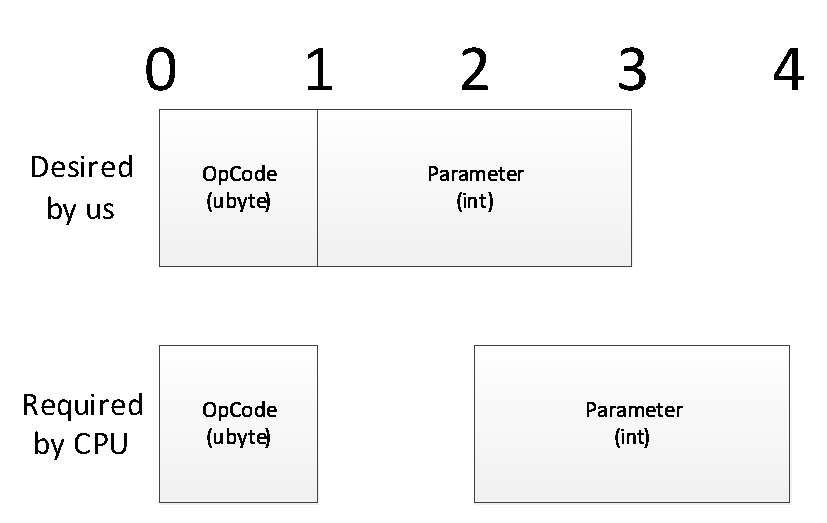
\includegraphics[scale=0.75]{Diagrams/byte-alignment.eps}
\caption{Alignment Issues}
\label{fig:alignment-issues}
\end{figure}

\begin{figure}[ht!]
\begin{verbatim}
[java] **** Illegal read - misaligned word from $2c01 at $80de
[java] Stack Trace: number of calls: 4 PC: $80de
[java] evaluate (errno.c) called from PC: $7166
[java] process_thread_mainProcess (local in pred-eval.c) called from PC: $bf12
[java] call_process (local in process.c) called from PC: $c0b2
[java] process_run (errno.c) called from PC: $4250
\end{verbatim}
\caption{Example of the error messages produced by MSPSim in Cooja that led to the discovery of this bug}
\end{figure}

As can be seen in \autoref{fig:alignment-issues} if we were to align the words as the CPU wanted the size of the bytecode would massively increase as every single byte bytecode would need to be padded by a byte to (i) make sure all bytecode entries were the same length and to ensure the word parameters are correctly aligned. To solve this issue instead of accessing the memory directly in the bytecode what can be done instead is to copy the memory out byte-by-byte into a correctly aligned block of memory and use that instead. As we copy out byte-by-byte and not by word we can access the memory correctly.

\subsection{Examples of Compiled Programs}

\begin{figure}[H]
\begin{minipage}{0.65\linewidth}
\hrule
\begin{lstlisting}[language=Hoppy]
[all]
function 1 as slot returning int in
    using Neighbours(2) as twohopn in
        @(x : twohopn ~
            slot(x) != slot(this)
        )
\end{lstlisting}
\begin{lstlisting}[language=Dragon]
//TARGETING all
//FUNC 1 AS slot
//STORING 2 IN twohopn
IVAR 1
IPUSH 1
IPUSH 0
ISTORE 1
start1: ALEN 255
INEQ
JZ end1
//slot(a[*1])
VIFAFC 1 255 1
//slot(this)
THISC 1
INEQ
AND
VIINC 1
JMP start1
end1: HALT
//VD 2 = 255
\end{lstlisting}
\hrule
\begin{lstlisting}[language=Hoppy]
[all]
function 0 as addr returning int in
function 1 as slot returning int in
    using Neighbours(1) as onehopn in
        @(a : onehopn ~
            @(b : onehopn ~ addr(a) != addr(b)
                => slot(a) != slot(b))
            & slot(a) != slot(this)
        )
\end{lstlisting}
\end{minipage}\hspace{1em}
\begin{minipage}{0.25\linewidth}
\begin{lstlisting}[language=Dragon]
//TARGETING all
//FUNC 0 AS addr
//FUNC 1 AS slot
//STORING 1 IN onehopn
IVAR 1
IPUSH 1
IPUSH 0
ISTORE 1
start1: ALEN 255
INEQ
JZ end1
IVAR 2
IPUSH 1
IPUSH 0
ISTORE 2
start2: ALEN 255
INEQ
JZ end2
//addr(a[*1])
VIFAFC 1 255 0
//addr(b[*2])
VIFAFC 2 255 0
INEQ
//slot(a[*1])
VIFAFC 1 255 1
//slot(b[*2])
VIFAFC 2 255 1
INEQ
IMPLIES
AND
VIINC 2
JMP start2
//slot(a[*1])
end2: VIFAFC 1 255 1
//slot(this)
THISC 1
INEQ
AND
AND
VIINC 1
JMP start1
end1: HALT
//VD 1 = 255
\end{lstlisting}
\end{minipage}
\caption{Compiled check for slot collisions. Using 2-hop information of \autoref{fig:two-hop-slot-pred-lang} on the left and using 1-hop information of \autoref{fig:one-hop-slot-pred-lang} on the right.}
\label{fig:two-hop-slot-pred-lang-compiled}
\end{figure}

Here we can see the vast difference that is caused by using a single loop versus a nested loop in a predicate. The single loop program that uses two hop information as an assembled binary size of 28 bytes, whereas the assembled size of the one hop information program has a size of 68 bytes. This program size may eventually become important when reaching the maximum allowed size of a single packet, as it is unlikely that a program like this will be able to go much over 100 bytes (without support for splitting the program up into multiple packets).

Also included in the programs are comments placed there by the compiler to indicate what the code is doing, the aim is that the developers will be able to manually tweak the code to try to reduce the size of it. Perhaps one of the startling differences is the benefit of some of the special array opcodes as can be seen in \autoref{fig:app2-pred-lang-compiled} which is only 13 bytes long. Without the \verb|AMEAN| opcode there would need to be a loop in IR to calculate the mean, by shifting this responsibility to the interpreter the code size can reduced by eliminating an interpreted loop.

\begin{figure}[H]
\begin{minipage}{0.7\linewidth}
\begin{lstlisting}[language=Hoppy]
[all]
function 2 as temp returning float in
    using Neighbours(2) as twohopn in
        abs(temp(this) - mean(temp, twohopn)) <= 10
\end{lstlisting}
\end{minipage}
\begin{minipage}{0.2\linewidth}
\begin{lstlisting}[language=Dragon]
//TARGETING all
//FUNC 2 AS temp
//STORING 2 IN twohopn
//temp(this)
THISC 2
AMEAN 255 2
FSUB
FABS
IPUSH 10
ICASTF
FLEQ
HALT
//VD 2 = 255
\end{lstlisting}
\end{minipage}
\caption{Compiled mean temperature check of \autoref{fig:app2-pred-lang}}
\label{fig:app2-pred-lang-compiled}
\end{figure}

One final optimisation that is worth mentioning is that, while we have support for it, we will often not generate code that involves pushing floats onto the stack. This is because if it is possible it we can save a byte of the program size by instead pushing an integer and then casting it to a float. When pushing a float we need 1 byte for the opcode and 4 bytes for the float being pushed giving 5 bytes of program. In the optimised case we need 1 byte for the \verb|IPUSH| opcode, 2 bytes for the integer and 1 byte for the \verb|ICASTF| opcode giving 4 bytes of program instead of 5.


\subsection{Testing}

As the virtual machine and its parsers can be fairly complex and difficult pieces of code to understand it was very important that we had test cases that validated that the functionality was correct. To do this three sets of tests are performed. Of them two are unit tests, one that tests that assembled bytecode can be correctly executed and the other that tests that the parser/compiler can correctly parse and generate code. After this is an integration test, that checks if the output of the parser/compiler converted into bytecode by the assembler can be correctly executed. To test the correct execution set data is given to the virtual machine, which can then be used in the predicates.

Different things are tested for each of the integration tests. When testing the assembler and virtual machine, short programs of opcodes are provided to test simple activities such as pushing onto the stack, calling functions or arithmetic. This is simply to test the functionality of the virtual machine. As we can be sure that the functionality is correct, when testing the compiler more complex predicates that we have designed the system to use are tested. We expect that for some of these tests scripts the code would be the same for real world uses.



\subsection{Data Transmission}

So far we have covered what we wish to evaluate and how that shall be evaluated, however, we have not talked about how data shall reach its destination to be evaluated. The how of evaluating data is split into two parts: `where' the predicate should be evaluated and `when' the data should be disseminated.

Regarding where a predicate should be evaluated there seem to be two choices. Either there is collection of all the networks state at a single location designated as a sink (such as the base station), this is what traditional Global Predicate Evaluation algorithms would do. Or, the predicate could be evaluated in the network at some target node. We intend to investigate both of these.

Considering when the data should be disseminated there are again several options available. The first and most obvious is to simply periodically send out the information. However, periodic data transmission could potentially inefficient, so we will also investigate event-based dissemination. Finally, nodes could also request information when it is desired. We investigate all three of these.

\begin{table}[H]
\centering
\begin{tabular}{| l | m{5cm} | m{5cm} |}
\hline
~ & Local & Global \\
\hline
Periodic & Periodically asks neighbours for information & Periodically aggregates information to sink \\
\hline
Event & Periodically checks for changes, on change floods information locally &  Periodically checks for changes, on change aggregates data to sink \\
\hline
\end{tabular}
\caption{Description of predicate evaluation behaviours}
\end{table}


\subsubsection{Local Event}

When gathering data in-network using an event-based update mechanism and evaluating the predicate locally in-network there two things of importance. The first and simplest is knowing that data has changed. Because there are no ways to plug into the OS and receive notifications that a section of memory has changed it means that the local data needs to be checked periodically for a change. To do this the function that the library user has provided to return the node data will be called and then compared against some history. This history is simply the last piece of data that was sent into the network. A comparison function needed to be supplied by the user because doing a simple comparison of the memory may lead to change events being fired even though values have not changed. There are several examples where this is important. The first is that floating point calculations can produce different representations of the same results, bitwise the values may differ but logically the values are the same. Another case is that many sensors have a tolerance associated with them, by checking the values with a function this tolerance can be taken into account and events will not be fired if the data has not changed significantly. Finally, using a tolerance function allows the library user to specify the difference that is meaningful to them, even if it is different to the sensor tolerance.

As we check periodically to detect a change and then fire events, it means that there is still the possibility that we will miss some changes. For example a sensor value may spike in between measurements and this may never be detected due to how the checking period aligns with the spikes.

When an event is fired that indicates that the node's data has changed it means that the data will need to be sent to some of the nodes in the network. Our implementation simply floods the information the maximum number of hops a predicate is asking for data. For example if there are 3 predicates in the network using 1-hop, 2-hop and 4-hop data, every node will flood their data 4-hops when it changes. This solution works because every node keeps a record of all the predicates in the network even if they are not evaluated by every node.

There is the potential for optimisations here by using knowledge of the node's neighbours to detect if a node actually needs the current nodes data and then only flooding the data if that is the case. For example if there is one predicate in the system that is targeted to a single node that needs 3-hop information, but the node whose data has just changed is 4 hops away, that node would not need to send its information. However, this would mean that every node would need an accurate picture of the network state. This may be energy intensive to calculate, so we leave this optimisation to be investigated in later work.

\begin{figure}[H]
\centering
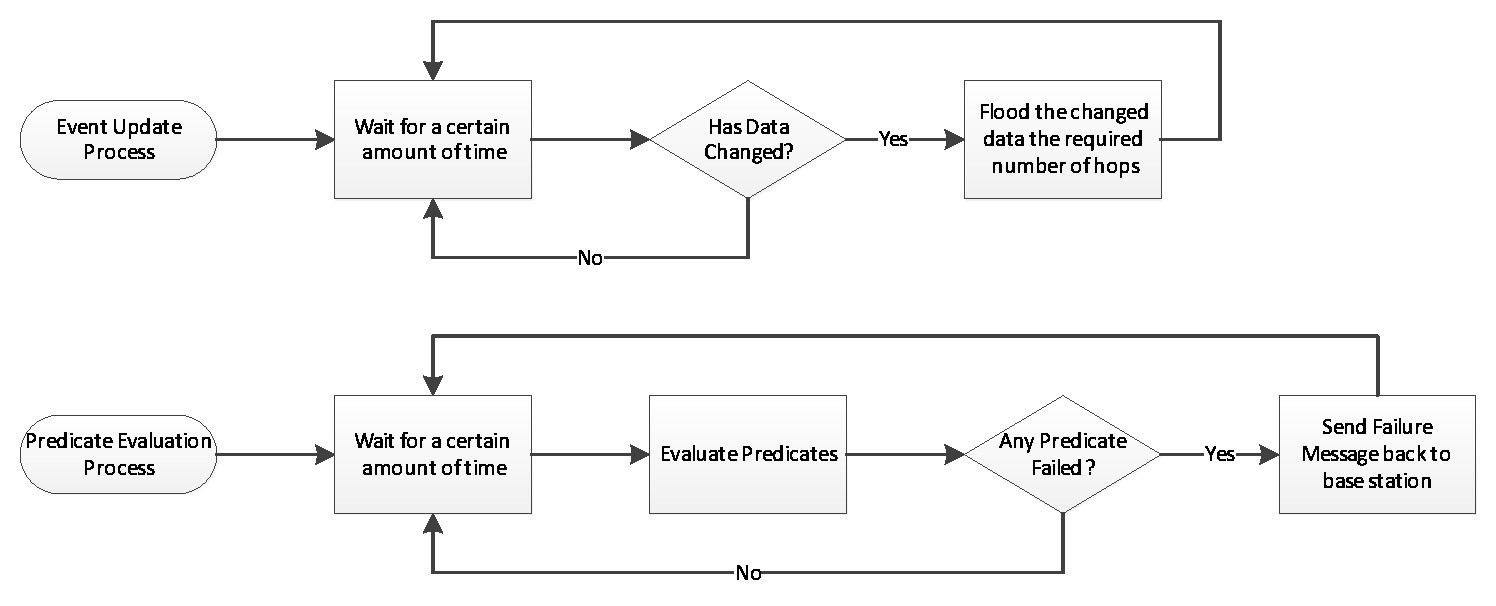
\includegraphics[width=\linewidth]{Diagrams/pele.eps}
\caption{Predicate Evaluation Local Event (PELE)}
\end{figure}

\subsubsection{Local Periodic}

The major difference between evaluating data periodically when evaluating a predicate in-network is that instead of data being sent to nodes when it changes, data is only sent to nodes when it is requested. The idea is that when a node is evaluating its predicates it finds the maximum distance it needs information for and floods a message that many hops asking for data and each of those nodes reply back along the path that the request message came from. After a node evaluates all its predicates for that period it then forgets all that information. The reason this is done is because in the event based dissemination there is no ability to detect changes in topology and remove invalid data. For example say a cluster head that has successfully delivered information in the past crashes. As that information has been delivered and is only updated when it changes all the nodes simply assume that the data remains the same and will continue evaluating the predicate as if the cluster head had not crashed. Neighbours of the failed cluster head could detect and send this information, but as that involves network information it is not an application predicate and is out of the scope of this work. So the solution was to simply consider the information available at the node evaluating a predicate at that instant.

Instead of requesting information every node could simply periodically broadcast it. However, that has the disadvantage of causing nodes to broadcast information when they don't need to (a problem from event-based dissemination) and also could lead to problems when nodes clocks are perfectly aligned. For example nodes could consistently receive old information from nodes if they keep sending data that was meant for a previous round such that is it only received during the current round of predicate evaluation. By asking for data these issues are mitigated.

\begin{figure}[H]
\centering
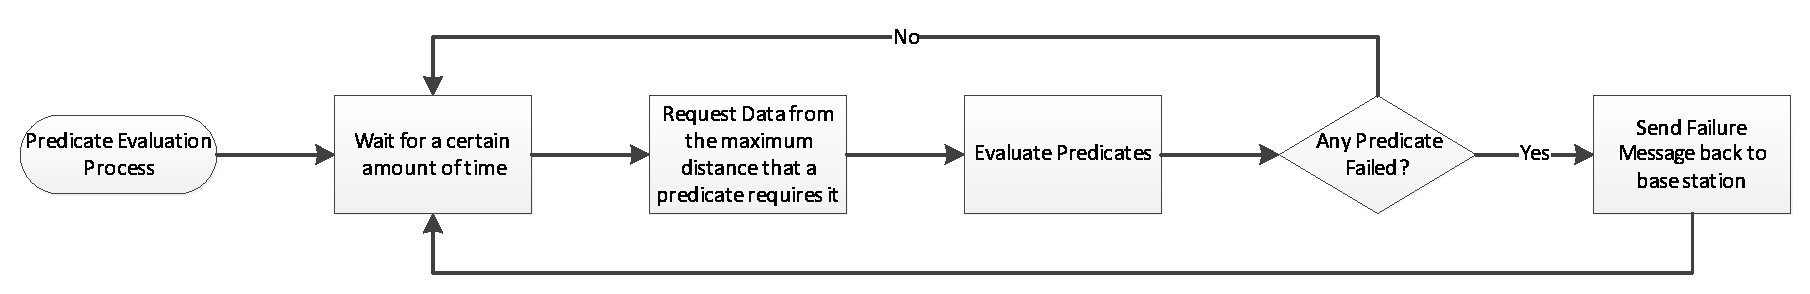
\includegraphics[width=\linewidth]{Diagrams/pelp.eps}
\caption{Predicate Evaluation Local Periodic (PELP)}
\end{figure}

When using the N-Hop Request library to implement this predicate evaluator there is an important issue that needs to be considered: when we have sent the data request message how long should we wait for? We cannot simply wait until all the results are returned to the evaluating node because (i) we do not necessarily know what node's data we will be waiting for and (ii) we may not receive that data anyway. We could wait for $2 \times D \times T_{send} + \epsilon$ time units, where $D$ is the maximum number of hops we are asking for information from, $T_{send}$ is the amount of time it takes for a message to try to be sent and $\epsilon$ is a small extra amount of time to wait. However, knowing what $T_{send}$ is can be difficult, and is based on many complicated factors. For example, if the MAC protocol in use uses CSMA/CD or CSMA/CA then it is possible, when trying to send a message, to enter into an arbitrary number of back-off period while waiting for the channel to be free \cite{?}. If there is an upper bound on the number of retries then we can calculate a maximum $T_{send}$, otherwise we cannot. Therefore, for our implementation we chose to use a fixed large value in which it was reasonable to expect all the responses that would return, would return within that period. We expect that in the future, this wait period will need to be some function of $D$ the number of hops of information being asked for to support requesting information from deeper in the network.


\subsubsection{Global}

When considering evaluating predicates at a sink, the data can simply be aggregated to it along a tree. For both event-based and periodic data generation the way the data is generated can remain the same, the requesting of data is simply removed (for periodic) and instead of flooding the information to neighbours it is aggregated instead.

However, this change causes a few knock-on effects. For the aggregation of neighbours and data in PEGP the behaviour is as expected, data is generated at the leaves and aggregated onwards towards the tree's root node where it is used. When aggregating data that is generated in PEGE, it is not the leaves that periodically generate data. Instead every node could potentially cause a message to being being forwarded through the tree. The big change is that every time a packet is forwarded the current node's data is aggregated to with it. This means that nodes closer to the root node of the tree have more opportunities to aggregate their data. Overall we do not believe this will affect the evaluation behaviour, as in the worst case more recent information may be available when it might not otherwise have been so.

The biggest issue with the global style of predicate evaluation is the latency that is introduced between gathering the data from the nodes in the network and the evaluation of the predicate. One problem is that the data in the network may have changed since it was gathered, a larger problem is that data will be compared at potentially very different times due to the aggregation delays. This was not as much of an issue with local in-network evaluation because the data was quickly flooded back to the target node. However, with tree aggregation every hop towards the sink needs a long wait to gather as much data as possible to reduce number of messages sent. This could potentially lead to a number of predicates being incorrectly evaluated by using data from different times.

\begin{figure}[H]
\centering
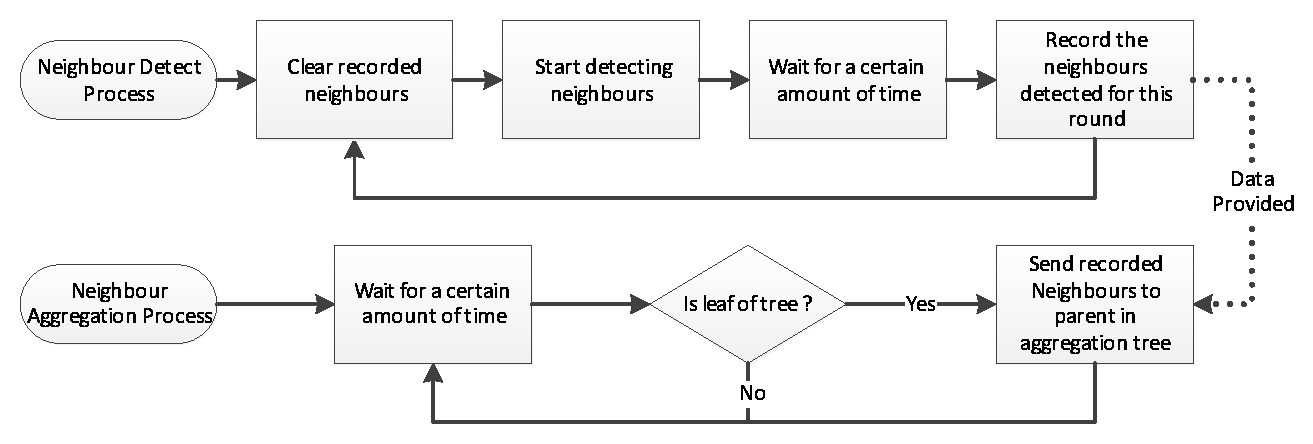
\includegraphics[width=\linewidth]{Diagrams/pegx-neighbour-agg.eps}
\caption{Neighbour Aggregation used for global predicate evaluation}
\end{figure}

Both the event-based and period versions of global predicate evaluation require the two processes of neighbour detection and aggregation running. Initially we planned to use this data to visualise the state the network is in. However, it turns out that it is a vital component of global predicate evaluation. Without this information we would be unable to work out how many hops  the data is from the node that is currently being evaluated.

As every predicate is evaluated is evaluated at the root of the aggregation tree, it becomes necessary for that root node to be able to pretend that they are the node where the predicate would usually have been evaluated. This is so the relevant neighbours can be used, and also so the virtual machine will use the correct data for the $this$ variable.

\begin{figure}[H]
\centering
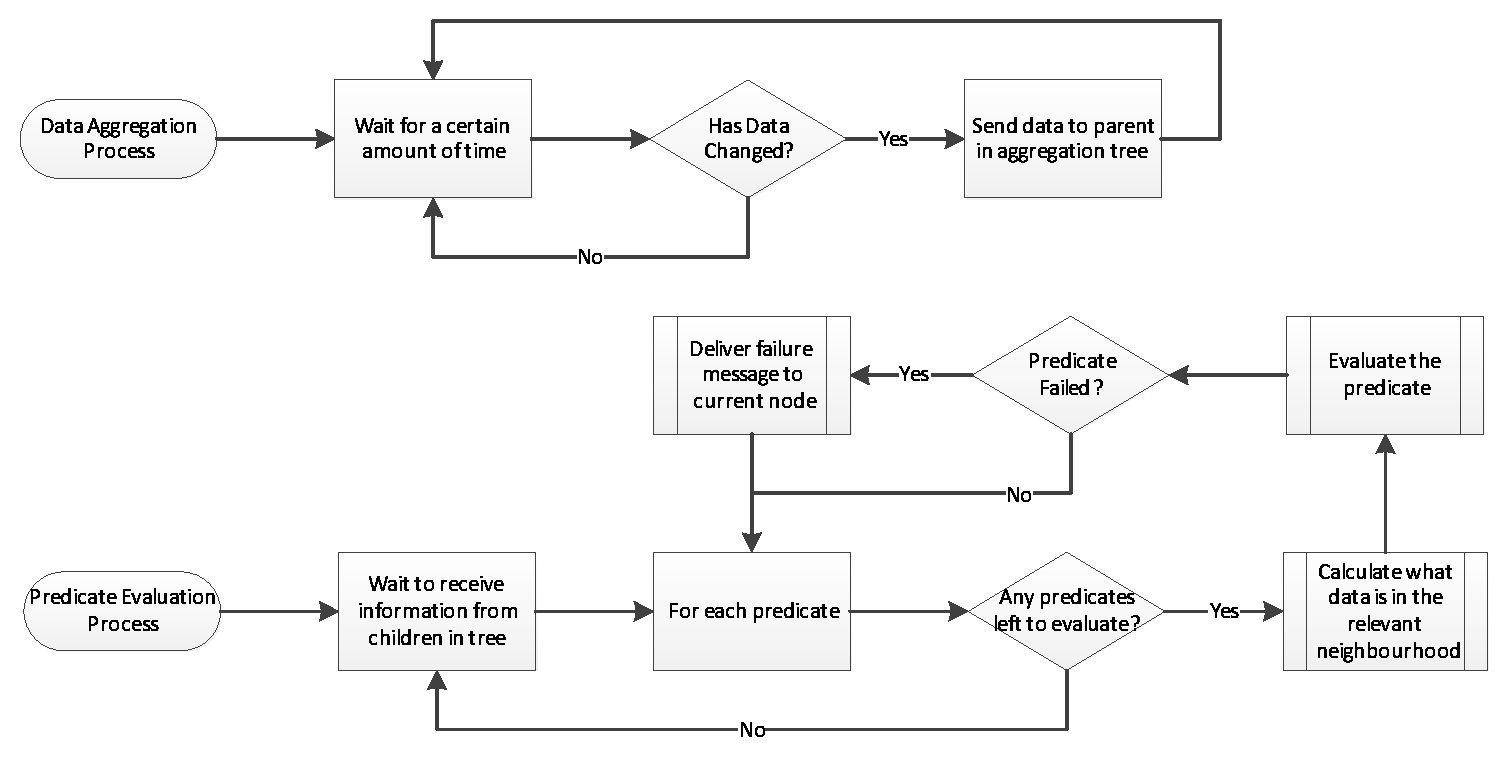
\includegraphics[width=\linewidth]{Diagrams/pege.eps}
\caption{Predicate Evaluation Global Event (PEGE)}
\end{figure}

Between the two versions of global predicate evaluation there are only minor differences in how the algorithm is implemented. The first is that when sending data PEGE checks to see if the data has changed before sending it, PEGP instead checks if the node is a leaf in the tree and relies on the aggregation of intermediate nodes to gather all the network's data. The second is a consequence of the first difference, PEGE will keep and update the information it receives. PEGP instead only used the last round of information that has been received. So after every predicate has been evaluated at the end of a predicate evaluation round the node information is cleared. This feature was added to enable support for (untested) handling failures in the network such as crashes or for handling the case when the nodes are mobile.

\begin{figure}[H]
\centering
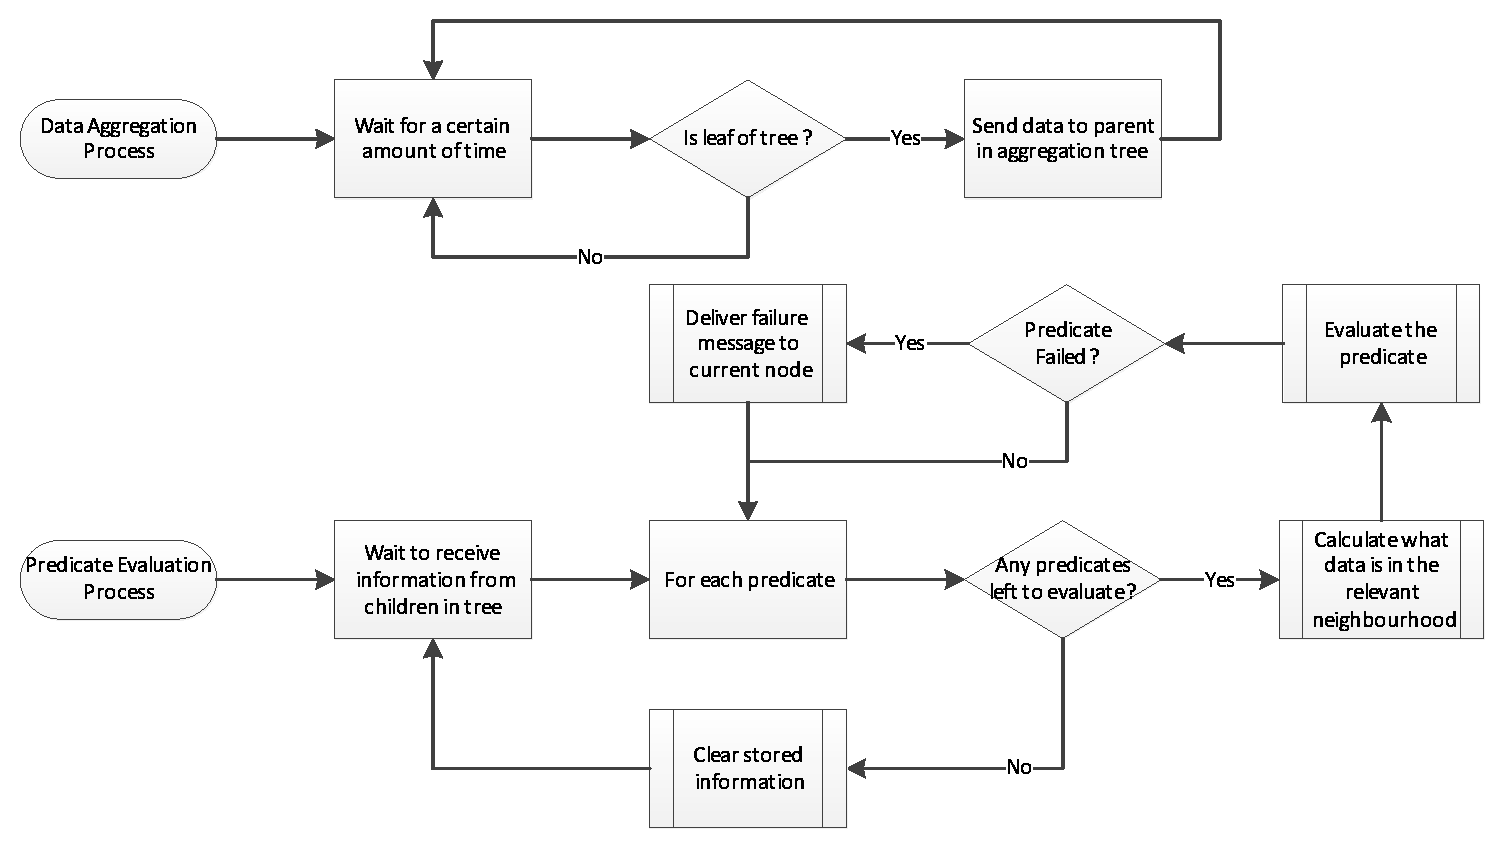
\includegraphics[width=\linewidth]{Diagrams/pegp.eps}
\caption{Predicate Evaluation Global Periodic (PEGP)}
\end{figure}


\subsubsection{Reply}

Once a node has reached the point of having a result after evaluating a predicate it needs to do something meaningful with that information so that users looking for results at the base station also end up knowing this information. The first and most obvious solution would be to inform the base station of every result, be it success or failure. Unfortunately while this is the most comprehensive response it is would also require the most energy as every node would need to send a repose message for every predicate they were evaluating.

\begin{equation}
C = |P_{all}| \times |V| + |P_{single}|
\end{equation}

The alternatives are to either send a message when a predicate has failed or when a predicate succeeds. This allows only a fraction of $C$ messages to be sent. However, there are a number of differences that make deciding to send success or failure an important decision. First of all is how the result is represented. The comprehensive solution has the advantage that the result of a predicate can be put into an \emph{unknown} state. Once a result message is received the result of that predicate can be moved into a \emph{failed} or \emph{succeeded} state. For success or failure messages you would need to assume the opposite of the messages that you are waiting for (i.e. assume predicates failed before receiving the succeeded message and vice versa) and change the state once the message is received. If messages are lost then this will lead to false notifications of success when waiting for failure messages and false failures when waiting for success messages.

The other issue to consider is what should be reported. If success messages are the chosen form of the response, then what useful information could they contain? One would expect the state that the predicate was evaluated with, but this information is not nearly as useful as the state that caused a predicate to fail. Another factor is that to create a useful description of why an error message failed is complex and would require more resources than simply evaluating the message. This means that practically it would be best for a failure message to report the state that caused the predicate to fail back to the base station and then expect further analysis on it there.

As we expect a predicate failure to be an infrequent event, our libraries have been designed to report only predicate failures. This should save energy in the form of messages. However, we expect the system to be vulnerable to not showing the full extent failures (falsely appearing successful), when messages are lost.


\subsection{A Consideration}

One of the main examples provided was the problem of assigning slots in a TDMA MAC protocol, where one would wish to ensure that no node within two hops of any given node has the same slot. Interestingly there are multiple ways to structure the predicate to perform this evaluation.


The first predicate we might consider is the one where for every node, we get the 2-hop neighbourhood and check that none of those nodes have the same slot as the initial node. This means that we would need to send:
\begin{enumerate}
	\item A message from the base station to the node asking it to evaluate the predicate
	\item A message from the node to each of its 2-hop neighbours
	\item Each 2-hop neighbour needs to send a message back to the node
	\item The node would need to wait for its neighbours to send the messages, then evaluate the predicate. This would imply that the node would need to know who is in its two hop neighbourhood
	\item The node would need to report to the base station the result of the predicate
\end{enumerate}

So we would need at best $|V| + \Delta_{sink}(n) + M(P)$ messages to evaluate this predicate for the single node $n \in V$. We need $|V|$ message to flood the predicate to every node, $\Delta_{sink}(n)$ is needed to send a failure reply back to the sink and the last component $M(P_{2})$ is the message cost of evaluating the predicate on that node. For example $M(P_{2}) = 2|Neighbours(n, 1)|$ for PELP as a message has to be flooded out two hops to ask for the information and then those nodes need to respond.

\begin{align}
\label{eq:2-hop-slot-pred}
& 				\forall n \in \text{Nodes} \cdot \\
& \hspace{2em}		\forall n' \in \text{Neighbours}(n, 2) \cdot \\
& \hspace{4em}			\text{slot}(n) \neq \text{slot}(n')
\end{align}

The second predicate we could consider is the one where every node checks their 1-hop neighbourhood for slot collisions. Here we model the 2-hop nature of the predicate differently, because instead of checking on the node that we want to check for slot collisions, we check on the node between two nodes that might have slot collisions.

\begin{enumerate}
	\item A message from the base station to the nodes adjacent to that we asking to check slot collisions
	\item A message from the node to each of its 1-hop neighbours
	\item Each 1-hop neighbour needs to send a message back to the node
	\item The node would need to wait for its neighbours to send the messages, then evaluate the predicate. This would imply that the node would need to know who is in its two hop neighbourhood
	\item The node would need to report to the base station the result of the predicate
\end{enumerate}

Initially one may consider that this 1-hop predicate can simply be evaluated on a node $n' \in V$ where $\{n, n'\} \in E$. However, this means that this predicate is no longer equivalent to that 2-hop predicate. For example if $n$ has another neighbour $n''$ whose 1-hop neighbourhood is not contained within $n'$'s 1-hop neighbourhood ($Neighbours(n'', 1) \setminus Neighbours(n', 1) \not= \emptyset$) then $n''$ would also need to be checked.

So the number of message that would be required to evaluate this 1-hop predicate on the required node is  $|V| + \sum_{n' \in Neighbours(n, 1)}{\Delta_{sink}(n')} + M(P_{1})$. Where $|V|$ is required for the same reasons as the 2-hop predicate and every neighbour $n'$ of $n$ needs to send a failure message. $M(P_{1}) = \sum_{n' \in Neighbours(n, 1)}{2|Neighbours(n', 1)|}$ for PELP because every neighbour $n'$ of $n$ needs to ask $n'$'s 1-hop neighbourhood for information.


\begin{align}
\label{eq:1-hop-slot-pred}
&				\forall n \in \text{Nodes} \cdot \\
& \hspace{2em}		\forall n' \in \text{Neighbours}(n, 1) \cup \{n\} \cdot \\
& \hspace{4em}			\forall n'' \in \text{Neighbours}(n, 1) \cup \{n\} \cdot \\
& \hspace{6em}				\text{addr}(n') \not= \text{addr}(n'') \implies \text{slot}(n') \neq \text{slot}(n'')
\end{align}

So this introduction of the 1-hop predicate has led to a spreading out of the evaluation, but with roughly the same amount of energy usage. The energy usage is roughly the same as the number of nodes from which data is requested is the same in $M(P_{1})$ as $M(P_{2})$. However, the 1-hop implementation has a good advantage, which is that by asking nodes neighbouring the 1-hop neighbours of $n$ to also evaluate the predicate they can take advantage that some of the predicate is already being evaluated. As shown in \autoref{fig:1-hop-new-eval} a new node can be set to evaluate a predicate and that node will take advantage of the already evaluated neighbouring information that is not necessary to repeat. Whereas the 2-hop predicate would need to repeat a lot of data request and evaluation if it were to be evaluated on multiple nodes. So Adding more and more nodes that evaluate the 1-hop predicate will scale much better than the 2-hop predicate simply because the of way that the evaluation is distributed and the way that distribution can prevent duplicate requesting of information. So checking an entire network for slot collisions should be much more energy efficient when using the 1-hop predicate.


\begin{figure}[H]
\centering
\subfigure[Checking green node has no slot collisions]{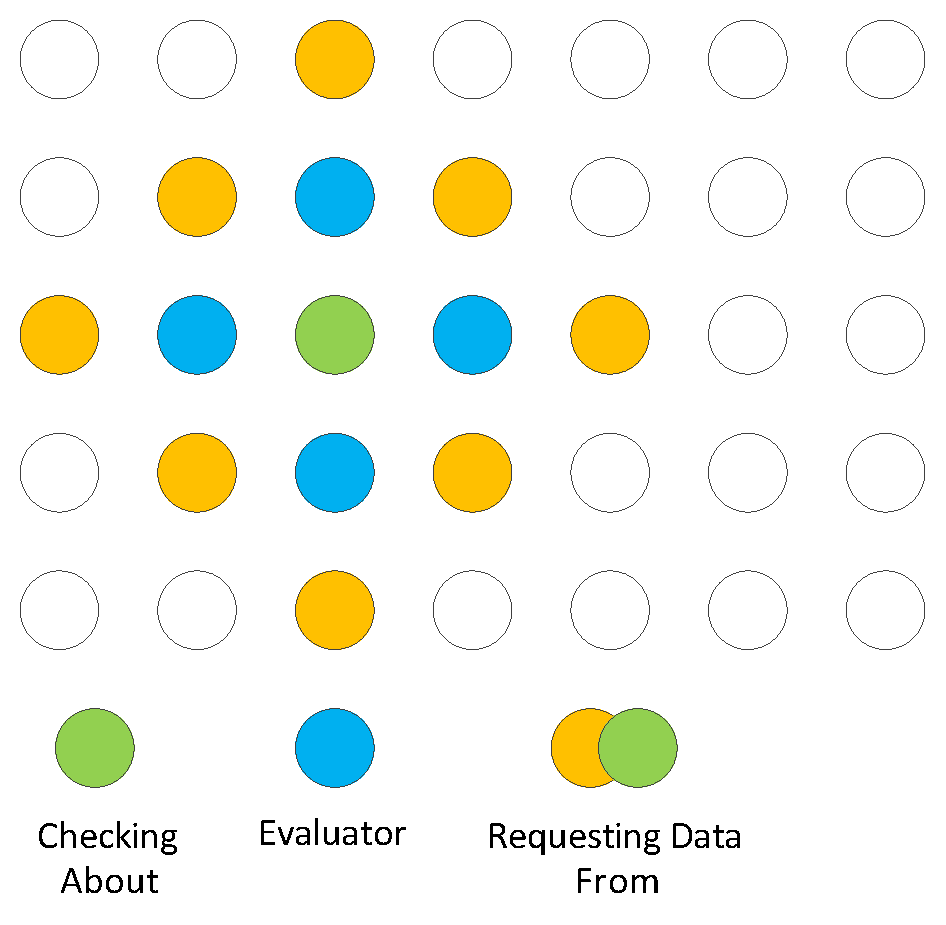
\includegraphics[width=0.4\linewidth]{Diagrams/1-hop-checking-a.eps}}\hspace{3em}
\subfigure[Adding new evaluators to check new node has no slot collisions]{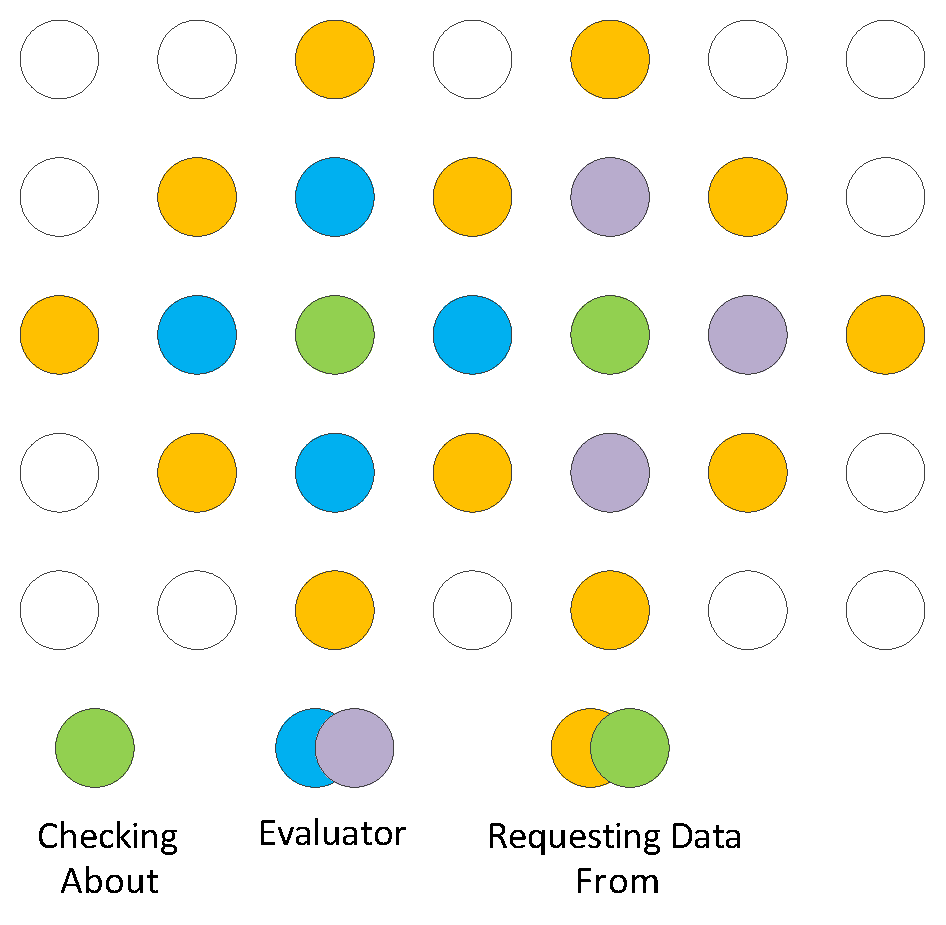
\includegraphics[width=0.4\linewidth]{Diagrams/1-hop-checking-b.eps}}
\caption{Utilising the 1-hop predicate structure to add new evaluators}
\label{fig:1-hop-new-eval}
\end{figure}


However, there is one final factor to take into account that even though using 2-hop information will require more energy it is the simpler predicate - it only has a single loop with a simpler check. This predicate requires 28 bytes instead of the 68 bytes that the predicate that required 1-hop information uses. When predicates get larger and more complicated it may be important that they can be expressed in a simpler way that may perhaps use more energy, but also are smaller and need less stack space to be evaluated. If the cost of performing a firmware update across the network is very high and would be needed to support larger predicates, then the energy cost of the simpler predicate may end up being worth it.

\subsection{A Distance Issue}

% Problem of Distance(n, n')

The only network primitive we have implemented is a function that gets information on nodes within a certain number of hops of the asking node. There are a number of other network primitives that might be useful for both network and application predicates. One of these is the ability to get the distance between two nodes.

An example of a predicate that uses $Neighbours(n, h)$ is shown below. This predicate is for Hierarchical Clustering where $H$ is a parameter that defines the distance between cluster heads. The predicate checks that for every node there is a neighbour in the $H$-hop neighbourhood that is a cluster head.

\begin{align*}
& \hspace{2em}	\forall n \in Nodes \cdot \\
& \hspace{4em}		\exists n' \in Neighbours(n, H) \cdot \\
& \hspace{6em}			IsClusterHead(n)
\end{align*}

An alternative way that we might specify this predicate is to check that the distance between a node and the cluster head (that it knows the address of) is within $H$ hops.

\begin{align*}
& \hspace{2em}	\forall n \in Nodes \cdot \\
& \hspace{4em}		IsClusterHead(n) \lor Distance(n, ClusterHead(n)) \leq H
\end{align*}

However, there is an issue with this predicate. How would we implement the $Distance(n, n')$ primitive? With $Neighbours(n, h)$ we know how far we need to ask for information ($h$ hops), with $Distance(n, n')$ the maximum distance that we will need to wait for information to return from is the diameter of the network. Unfortunately we cannot assume that the diameter is known. If instead we take a time-out approach there is no way that we can guarantee to wait for the correct amount of time. For example if we wait enough time to check if a node is at maximum $D$ hops from the given node the node will need to wait for  time units. However, if the node we are trying to find the distance of is at $D + 1 $ hops then we will not believe the two nodes are connected. To reliably wait to check if two nodes are connected in a network where the diameter is not known we will need to wait for $\infty$ time units. Thus making $Distance(n, n')$ impossible to implement without knowing the diameter. Due to this issue we have not implemented such a network primitive function.


\subsection{Optimising on Predicate Structure}

% Conjuntive vs disjuntive predicates


When evaluating predicates in-network, it possible to consider optimisations due to the structure of the predicate to reduce the amount of information that is requested. For example take conjunctive predicates where the structure of the predicate $P$ is $P = P_1 \land P_2 \land \ldots \land P_n$. If one of the $P_i$ is false then the result of the predicate $P$ is false ($False \land P \Leftrightarrow False$). This means that the statements could potentially be evaluated in an order such that the $P_i$ that requires the fewest resources is evaluated first and the $P_j$ that requires the most resources is evaluated last.

The aim of this optimisation is to reduce energy usage by sending fewer messages. For the two types of data gathering in-network and at the sink, when gathering this data at the sink it would not be of any use as the data is sent to the sink in an event-based or periodic way. The sink doesn't ask for this information, so it is not possible for it to not ask for certain pieces of data. This is also true of event-based in-network predicate checking. So the only time this optimisation would be of use to us is when gathering data for in-network predicates that are checked periodically.

%Surprisingly, asking for and receiving all the required information actually requires fewer messages than incrementally asking for information. This is because of the communication that needs to be repeated when asking for more information. For example if you have a conjunctive predicate where the sub-predicates require 1 and 3 hops of information. If we ask for all information then we simply send messages out 3 hops and then receive replies from all the nodes in that neighbourhood. If we instead ask for one-hop information first and then three-hop, we first have to send a message to local neighbours and then will end up sending them another data request message when asking for three-hop information (as the 1-hop neighbourhood is contained within the 3-hop neighbourhood).

For some predicates it may make obvious sense to implement such an optimisation, such as if there is a conjunctive predicate that needs 1-hop information and 15-hop information. If the 1-hop predicate is often false, then it saves asking for information from all nodes that are within 15 hops of the evaluating node. However, as many of the predicates are not likely to require information from that distance (we expect one to two hops, with the possibility of three hops) it is an optimisation that would not serve to optimise what we are targeting our system to evaluate. Another issue is that many of the predicates we have thought up are not of this form, they mostly have quantifiers as the outer structure with other logical operators inside that quantifier. It may be the case where you have a predicate of the following structure $P = P_{local} \land \land P_{network}$ where $P_{local}$ needs no network information, here there is the possibility to optimise the network request out if $P_{local}$ is false. However as adding this feature would increase the firmware size we decided against adding more optimisations. This was because the software began to reach the limit of the firmware size when the virtual machine was integrated with the message communication. However, investigating these kinds of optimisations is a future possibility.

%
%\begin{figure}[H]
%\begin{equation}
%\sigma(x) = \sum_{i=1}^{x} i \times |N(i)|
%\end{equation}
%\caption{The number of messages required to respond x hops}
%\end{figure}
%
%The sigma function is defined as it is because for each of the nodes that are $x$ hops away they will require sending their data message $x$ hops to reach the requesting node.
%
%\begin{figure}[H]
%\begin{equation}
%\sum_{j \in H} |N_F(j)| + \sigma(j)
%\end{equation}
%\caption{Maximum number of messages for an incremental data request}
%\end{figure}
%
%\begin{figure}[H]
%\begin{equation}
%|N_F(\text{max}(H))| + \sigma(\text{max}(H))
%\end{equation}
%\caption{Number of messages for a complete data request}
%\end{figure}






